%
% Copyright(c) 2015 Taikai Takeda <297.1951@gmail.com> All rights reserved.
%

\def\ba{\bm{a}}
\def\bb{\bm{b}}
\def\bc{\bm{c}}
\def\bd{\bm{d}}
\def\be{\bm{e}}
\def\bg{\bm{g}}
\def\bh{\bm{h}}
\def\bi{\bm{i}}
\def\bj{\bm{j}}
\def\bk{\bm{k}}
\def\bl{\bm{l}}
\def\bn{\bm{n}}
\def\bo{\bm{o}}
\def\bp{\bm{p}}
\def\bq{\bm{q}}
\def\br{\bm{r}}
\def\bs{\bm{s}}
\def\bt{\bm{t}}
\def\bu{\bm{u}}
\def\bv{\bm{v}}
\def\bw{\bm{w}}
\def\bx{\bm{x}}
\def\by{\bm{y}}
\def\bz{\bm{z}}

\def\bA{\bm{A}}
\def\bB{\bm{B}}
\def\bC{\bm{C}}
\def\bD{\bm{D}}
\def\bE{\bm{E}}
\def\bF{\bm{F}}
\def\bG{\bm{G}}
\def\bH{\bm{H}}
\def\bI{\bm{I}}
\def\bJ{\bm{J}}
\def\bK{\bm{K}}
\def\bL{\bm{L}}
\def\bM{\bm{M}}
\def\bN{\bm{N}}
\def\bO{\bm{O}}
\def\bP{\bm{P}}
\def\bQ{\bm{Q}}
\def\bR{\bm{R}}
\def\bS{\bm{S}}
\def\bT{\bm{T}}
\def\bU{\bm{U}}
\def\bV{\bm{V}}
\def\bW{\bm{W}}
\def\bX{\bm{X}}
\def\bY{\bm{Y}}
\def\bZ{\bm{Z}}

\section{Pairwise HMM}
\label{sec:phmm}
Pairwise HMMとは2つのsequence data(DNAの塩基配列やタンパク質のresidue配列)の類似度をモデル化したHMMである.これはdiscrete HMMの拡張であると考えることができるが,一般的なdiscrite HMMとは出力が2つのシンボルの組になるという点で異なる.隠れ状態の状態遷移図は以下のようになる.$M$はMatch状態,$X,Y$はそれぞれの配列の挿入状態を表す.

\begin{figure}[]
  \centering
  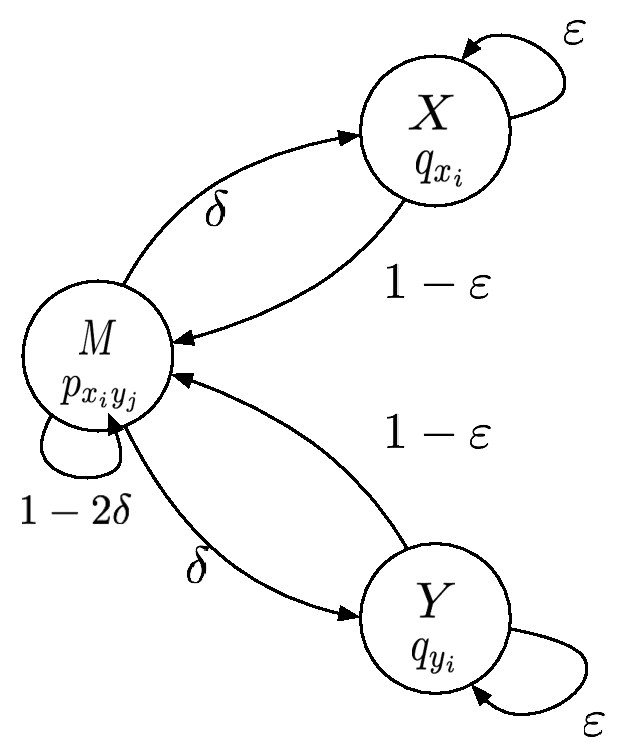
\includegraphics[width=0.3\textwidth, bb=0 0 300 400]{graffe/phmm_simple.pdf}  
  \caption{phmmの状態遷移図}
\end{figure}

\subsection{Notations}
\label{subsec:phmm_nt}
定式化する上でNotationを整理する.観測変数はシンボル列$\bm{x}, \bm{y}$である.
\begin{align}
\bm{x}&=(x^1,...,x^{T_x})\\
\bm{y}&=(y^1,...,y^{T_y})\\
\end{align}
観測変数$x^i, y^j$に対応する隠れ変数$\bm{z}^{ij}$は以下のように定義する.ここで,$x^i$もしくは$y^j$の代わりにgapを許す(観測されたシンボルが対応しない場合がある).
\begin{align}
\bm{z} = 
\begin{pmatrix}
\bm{z}^{11}  & \cdots & \bm{z}^{1 T_y} \\
\vdots  & \ddots & \vdots \\
\bm{z}^{T_x 1}& \cdots & \bm{z}^{T_x T_y}
\end{pmatrix}
\end{align}
隠れ変数は$\bm{z}^{ij}$は状態数$K$に対して1-of-$K$符号化方式で表される.
\begin{align}
\bm{z}^{ij} &= (z^{ij}_1,\ldots,z_K^{ij})\\
z_k^{ij} &= \left\{
\begin{array}{ll}
1 & \mbox{$x^i, y^j$は$k$番目の状態から出力される}\\
0 & \mbox{otherwise}
\end{array}
\right.
\end{align}
また,表記の簡単のため,$\bm{z}^{i0}=\bm{z}^{0j}=0$, 遷移の方向のoffsetとして$\bm{\delta}=\{(\delta_x, \delta_y)\}$と定義する.ここでは,$\bm{\delta}=\{(1,1),(0,1),(1,0)\}$となる.
これを用いて,隠れマルコフモデルの同時分布は以下ように表される.
\begin{align}
  p(\bm{x},\bm{y}, \bm{z}|\bm{\theta})=
p(\bm{z}^{11}|\bm{\alpha})
\prod^{T_x,T_y}_{i,j=1} \prod_{(\delta_x, \delta_y) \in \bm{\delta}}
 p(\bm{z}^{ij}|\bm{z}^{i-\delta_x, j-\delta_y}, \bm{\beta})
% \prod^{T_x,T_y}_{i,j=1}
%   p(\bm{z}^{ij}|\bm{z}^{i-1, j-1}, \bm{\beta})
%   p(\bm{z}^{ij}|\bm{z}^{i-1, j}, \bm{\beta})
%   p(\bm{z}^{ij}|\bm{z}^{i, j-1}, \bm{\beta})
\prod^{T_x,T_y}_{i,j=1}
  p(x^i y^j|\bm{z}^{ij}, \bm{\phi})
\end{align}
上記で,$\bm{\theta}=(\bm{\alpha},\bm{\beta},\bm{\phi})$はHMMのパラメタである.
\begin{align}
\begin{array}{ll}
\mbox{初期確率:}  & p(\bm{z}^{11}|\bm{\alpha})=\prod_{k=1}^K \alpha_k^{z_k^{11}}\\
\mbox{出力確率:}  & p(x^i, y^j|\bm{z}^{ij}, \bm{\phi}) = \prod_{k=1}^K p(x^i, y^j|\bm{\phi}_k)^{z^{ij}_k}\\
\mbox{遷移確率:}  & p(\bm{z}^{ij}|\bm{z}^{i-\delta_x, j-\delta_y}, \bm{\beta}) =  \prod_{l,k=1}^{L,K} \beta_{lk}^{z^{i-\delta_x,j-\delta_y}_l z^{ij}_k}
% & p(\bm{z}^{ij}|\bm{z}^{i-1, j-1}, \bm{\beta}) =  \prod_{k,l=1}^{K,L} \beta_{kl}^{z^{ij}_k z^{i-1,j-1}_l} \\
% &p(\bm{z}^{ij}|\bm{z}^{i, j-1}, \bm{\beta}) =  \prod_{k,l=1}^{K,L} \beta_{kl}^{z^{ij}_k z^{i,j-1}_l}\\
% &p(\bm{z}^{ij}|\bm{z}^{i-1, j}, \bm{\beta}) =  \prod_{k,l=1}^{K,L} \beta_{kl}^{z^{ij}_k z^{i-1,j}_l}
\end{array}
\end{align}
ここで,
\begin{align}
&\bm{\alpha} = (\alpha_1, \ldots, \alpha_K)\in\R^K\label{eq:res_a}\\
&\bm{\beta} =  (\bm{\beta_1}, \ldots ,\bm{\beta}_K)\in\R^K\times\R^K \mbox{ where } \ \bm{\beta}_k=(\beta_{k1},\ldots, \beta_{kK})\in\R^K\label{eq:res_b}\\
&\bm{\phi}  = (\bm{\phi}_1,\ldots,\bm{\phi}_K)
\end{align}
である.

\subsection{Biterbi Algorithm}

\subsection{EM algorithm}

\label{subsec:em}
EM algorithmによりパラメタの最適化を行う.EMアルゴリズムは以下のようなくり返しのアルゴリズムである.
\begin{align}
\mbox{\textbf{E-step}}&\\
&Q(\bm{\theta},\bm{\theta}^{old}) =
  \E_{p(\bm{z}|\bm{x}, \bm{\theta}^{old})}[\ln p(\bm{x}, \bm{z}| \bm{\theta})]\\ \\
\mbox{\textbf{M-step}}&\\
& \ \ \ \ \bm{\theta}^{new} \ \ \  = \argmax_{\bm{\theta}} p(\bm{\theta}, \bm{\theta}^{old})
\end{align}
Estepでは,事後分布$p(\bm{z}^{ij}|\bm{x})$と$p(\bm{z}^{ij}, \bm{z}^{i-\delta_x, j-\delta_y}|\bm{x})$を求める必要がある.
この事後分布はforward-backwardアルゴリズムで効率的に求めることが出来る.forward変数$
f$とbackward変数$b$を以下のように定義する.この2つの変数から,事後分布を求めることが出来る.ここでは,表記の簡単のためパラメタは明記しない.
\begin{align}
f^{ij} &= p(x^{1},\cdots,x^i, y^1,\cdots,y^{j}, \bm{z}^{ij})\\
b^{ij} &= p(x^{i+1},\cdots,x^{T_x}, y^{j+1},\cdots,y^{T_y}| \bm{z}^{ij})\\
\bm{\gamma^{ij}} &= p(\bm{z}^{ij}|\bm{x},\bm{y}) = f^{ij} b^{ij}/p(\bm{x},\bm{y})\\
\gamma^{ij}_k &= p(z^{ij}_k = 1|\bm{x},\bm{y})\\
\bm{\xi^{ij\delta}} &= 
p(\bm{z}^{ij}, \bm{z}^{i-\delta_x, j-\delta_y}|\bm{x},\bm{y}) = 
  f^{i-\delta_x, j-\delta_y} p(\bm{z}^{ij}|\bm{z}^{i-\delta_x, j-\delta_y}) p(x^{ij}|\bm{z}^{ij})b^{ij}  / p(\bm{x},\bm{y})\\
\xi^{ij\delta}_{lk} &= p(z^{ij}_k = 1, z^{i-\delta_x, j-\delta_y}_{l}=1|\bm{x},\bm{y})
\end{align}
ここで,表記の簡単のため$\bm{\gamma},\bm{\xi}$を定義した.すると,これらはDP(Dynamic Programming)で計算できる.
\begin{align}
f^{11} &= p(\bm{z}^{11})p(x^1,y^1|\bm{z}^{11})\\
f^{ij} &=
  p(x^i, x^j|\bm{z}^{ij})
  \sum_{(\delta_x,\delta_y)\in \bm{\delta}}  \sum_{\bm{z}^{i-\delta_x, j-\delta_y}}
  p(\bm{z}^{ij}|\bm{z}^{i-\delta_x, j-\delta_y})f^{i-\delta_x, j-\delta_y}\\
b^{T_xT_y} &= \bm{1} \\
b^{ij} &=
   \sum_{(\delta_x,\delta_y)\in \bm{\delta}}  \sum_{\bm{z}^{i+\delta_x, j+\delta_y}}
         p(x^{i+\delta_x}, x^{j+\delta_y}|\bm{z}^{i+\delta_x, j+\delta_y})
  p(\bm{z}^{i+\delta_x, j+\delta_y}|\bm{z}^{ij})b^{i+\delta_x, j+\delta_y}
\end{align}
Mstepでは,この事後分布$p(\bm{z}|\bm{x},\bm{y},\bm{\theta}^{old})$を用いてQ関数を最大化するパラメタ$\bm{\theta}$を求める.
\begin{align}
Q(\bm{\theta}, \bm{\theta}^{old})&=
\E_{ p(\bm{z}|\bm{x},\bm{y},\bm{\theta}^{old})}
[\ln p(\bm{x},\bm{y},\bm{z}|\bm{\theta})]\\
\bm{\theta}^{new} &= \argmax_{\bm{\theta}} Q(\bm{\theta}, \bm{\theta}^{old})
\end{align}
それぞれのパラメタは以下の通り計算できる.
\begin{align}
  \alpha_k &= \gamma^{11}_k / \sum_k \gamma^{11}_k\\
  \beta_{lk} &= \sum_{ij \bm{\delta}} \xi^{ij\delta}_{lk} / 
               \sum_{ij \bm{\delta}k}b\xi^{ij\delta}_{lk} \\
  \bm{\theta}^*_k &= \argmax_{\bm{\theta}_k} \sum_{ijk} \gamma^{ij}_k p(x_i, y_j|\bm{\theta}_k, z^{ij}_k = 1)
\end{align}
$\bm{\theta}$は,emissionの分布の形$p(x,y|\bm{\theta}, \bm{z})$を仮定することで得ることが出来る.ここでは,シンボルを$s^{1}...s^D$の$D$種類として,$s^m,s^n$の組み合わせを出力する確率を$\mu^{mn}$に持つ多項分布を仮定する.
\begin{align}
p(x,y| \bm{\phi}) = \prod_{mn} \mu_{mn}^{I(x, s^m) I(y, s^n)}
\end{align}
このとき,パラメータ$\bm{\phi} = \bm{\mu}$はラグランジュの未定乗数法を用いて以下のように求められる.
\begin{align}
  \mu^{mn} = \sum_{ij} \gamma^{ij} I(x^i, s^m) I(y^j, s^n)/ \sum_{ijmn} \gamma^{ij} I(x^i, s^m) I(y^j, s^n)
\end{align}
以上を用いて,パラメタの最適化を行うことができる.
